% Tier 1 result: online rho/IC ratio by panel, GitHub run 38523707244 (ubuntu-24.04).
% Data: ../tier1_github_38523707244/tier1_result.json (panels.A/B/C.primary). The two grey
% reference points are the earlier unisolated figures quoted in ../README.md (8.2x, and the
% 2026-10-12 crypto evaluation IC/strong = 1.38 [1.04, 1.88], i.e. rho/IC = 0.72 [0.53, 0.96]).
% Source of tier1_result.pdf; build: pdflatex tier1_result.tex
\documentclass[border=6pt]{standalone}
\usepackage{pgfplots}
\pgfplotsset{compat=1.17}
\begin{document}
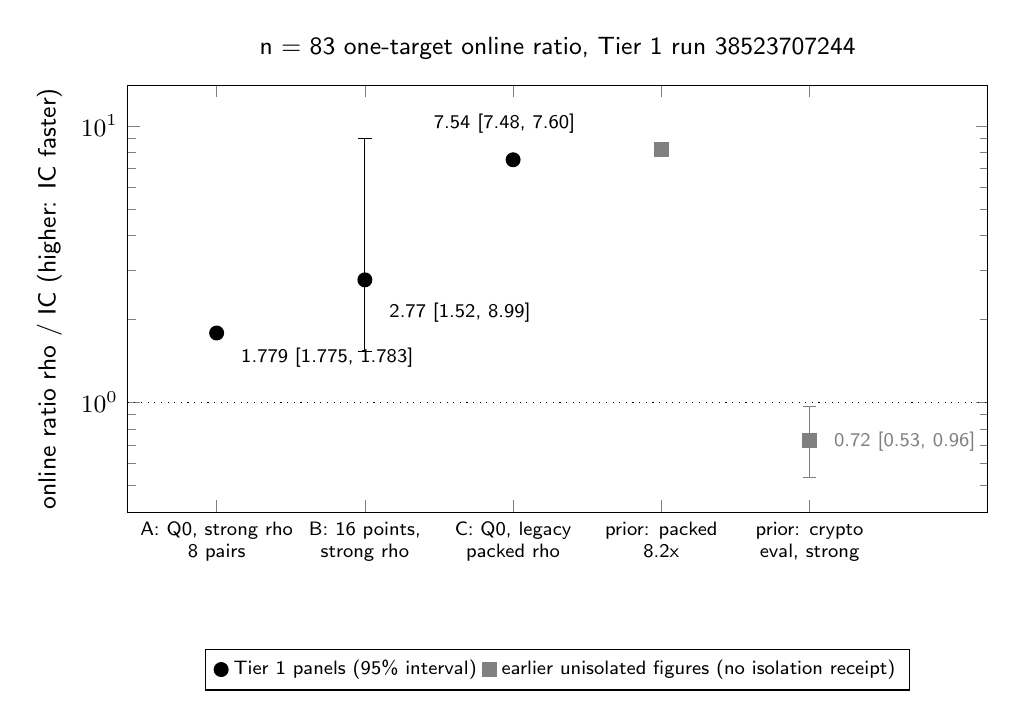
\begin{tikzpicture}[font=\sffamily\small]
\begin{axis}[width=12.5cm, height=7cm, ymode=log, ymin=0.4, ymax=14, xmin=0.4, xmax=6.2,
  xtick={1,2,3,4,5}, xticklabels={{A: Q0, strong rho\\8 pairs}, {B: 16 points,\\strong rho}, {C: Q0, legacy\\packed rho}, {prior: packed\\8.2x}, {prior: crypto\\eval, strong}},
  xticklabel style={align=center, font=\sffamily\scriptsize},
  ylabel={online ratio rho / IC (higher: IC faster)},
  title={n = 83 one-target online ratio, Tier 1 run 38523707244}, title style={font=\sffamily\small},
  legend style={at={(0.5,-0.32)}, anchor=north, legend columns=2, font=\sffamily\scriptsize}]
\addplot[only marks, mark=*, mark size=2.5pt, color=black, error bars/.cd, y dir=both, y explicit]
  table[x=x, y=y, y error plus=ep, y error minus=em] {
x y ep em
1 1.7786 0.0045 0.0040
2 2.7690 6.2207 1.2483
3 7.5357 0.0643 0.0596
};
\addplot[only marks, mark=square*, mark size=2.5pt, color=gray, error bars/.cd, y dir=both, y explicit]
  table[x=x, y=y, y error plus=ep, y error minus=em] {
x y ep em
4 8.2 0 0
5 0.7246 0.2400 0.1900
};
\draw[dotted] (axis cs:0.4,1) -- (axis cs:6.2,1);
\node[anchor=west, font=\sffamily\scriptsize] at (axis cs:1.1,1.45) {1.779 [1.775, 1.783]};
\node[anchor=west, font=\sffamily\scriptsize] at (axis cs:2.1,2.1) {2.77 [1.52, 8.99]};
\node[anchor=west, font=\sffamily\scriptsize] at (axis cs:2.4,10.2) {7.54 [7.48, 7.60]};
\node[anchor=west, font=\sffamily\scriptsize, text=gray] at (axis cs:5.1,0.72) {0.72 [0.53, 0.96]};
\legend{Tier 1 panels (95\% interval), earlier unisolated figures (no isolation receipt)}
\end{axis}
\end{tikzpicture}
\end{document}
